\documentclass[11pt,a4paper]{article}
\usepackage[left=2cm, text={17cm,24cm}, top=3cm]{geometry}
\usepackage[czech]{babel}
\usepackage[utf8]{inputenc}
\usepackage{times}
\usepackage[unicode]{hyperref} %pro křížové odkazy
\usepackage{graphicx} %pro práci s obrázky
\usepackage{float}
\usepackage[table,xcdraw]{xcolor} %barvičky
\usepackage{listings} %algoritmy, sazba kódu
\usepackage{algpseudocode}
\usepackage{pxfonts}
\usepackage{import}
\usepackage{multicol}
\usepackage{pdflscape}
\usepackage{multicol}
\usepackage{paracol}
\usepackage{enumitem}
\usepackage{longtable}

\graphicspath{{images}}

\definecolor{codegreen}{rgb}{0,0.6,0}
    \definecolor{codegray}{rgb}{0.5,0.5,0.5}
    \definecolor{codepurple}{HTML}{C42043}
    \definecolor{backcolour}{HTML}{F2F2F2}
    \definecolor{bookColor}{cmyk}{0,0,0,0.90}  

\setlength{\columnsep}{2pt}
\lstset{
        language = SQL,
        backgroundcolor=\color{backcolour},   
        commentstyle=\color{codegreen},
        keywordstyle=\color{codepurple},
        numberstyle=\footnotesize\color{codegray},
        stringstyle=\color{codepurple},
        basicstyle=\footnotesize,
        breakatwhitespace=false,         
        breaklines=true,                 
        captionpos=b,                    
        keepspaces=true,                 
        numbers=left,                    
        numbersep=-10pt,                  
        showspaces=false,                
        showstringspaces=false,
        showtabs=false,  
}

\begin{document}

\begin{titlepage}
    \begin{center}
        
\includegraphics[height = 160pt]{FIT_logo}\\
		
		{\Huge \textsc{Fakulta informačních technologií}\\[5pt]}
		{\Huge \textsc{Vysoké učení technické v~Brně}}\\
		\vspace{\stretch{0.382}}
		{\LARGE Databázové systémy\\[5pt]}
		{\LARGE Dokumentace k projektu IDS\\[30pt]}

    \end{center}
    \vspace{\stretch{0.609}}
    {
        \textbf{Pavel Osinek} (xosine00), \textbf{Adam Jetmar} (xjemta02)
		\hfill
		9. prosince 2021
	}
\end{titlepage}

\newpage
\tableofcontents
\newpage

\section{Zadání}
Na sociální síti bude možné uchovat veškeré základní informace o uživatelích
(včetně škol, bydliště, zaměstnání, kontaktu, vztahů, \dots). Uživatelé si mohou 
mezi sebou vytvářet (imaginární) přátelství pomocí žádosti. Každý uživatel
má svoji zeď, kde může on i jeho přátelé publikovat příspěvky, které budou 
mít obsah, datum, místo a čas publikování a můžou v nich být označeni i jiní 
uživatelé. Aby si uživatelé mohli sdílet nejen své příspěvky, ale také fotky,
mohou vytvářet i alba fotek, které budou mít svůj název, nastavení soukromí 
a popis. Na jednotlivých fotkách mohou být označení různí uživatelé a bude 
u nich uveden čas, datum a místo pořízení a jedna z fotek bude vždy titulní 
fotka alba. Navíc může být fotka pořízena v rámci nějaké akce. Uživatelé si 
mohou prostřednictvím konverzací s jistým názvem, do níž může být zapojen
jeden (on sám) a více uživatelů, vyměňovat zprávy, které budou mít svůj 
obsah, datum, čas a místo zaslání. Uživatelé mohou vytvářet akce, které se 
konají na určitém místě, v určitý čas a den a mohou mít nastavenou kapacitu (pokud není nastavena, kapacita je neomezená). Účastníci akce by měli znát, o 
jakou akci se jedná a pokud se jim akce zalíbí, tak se mohou akce, ať už jen 
virtuálně, či skutečně zúčastnit.
        
\section{Databázový model a model případů užití}
\begin{figure}[H]
  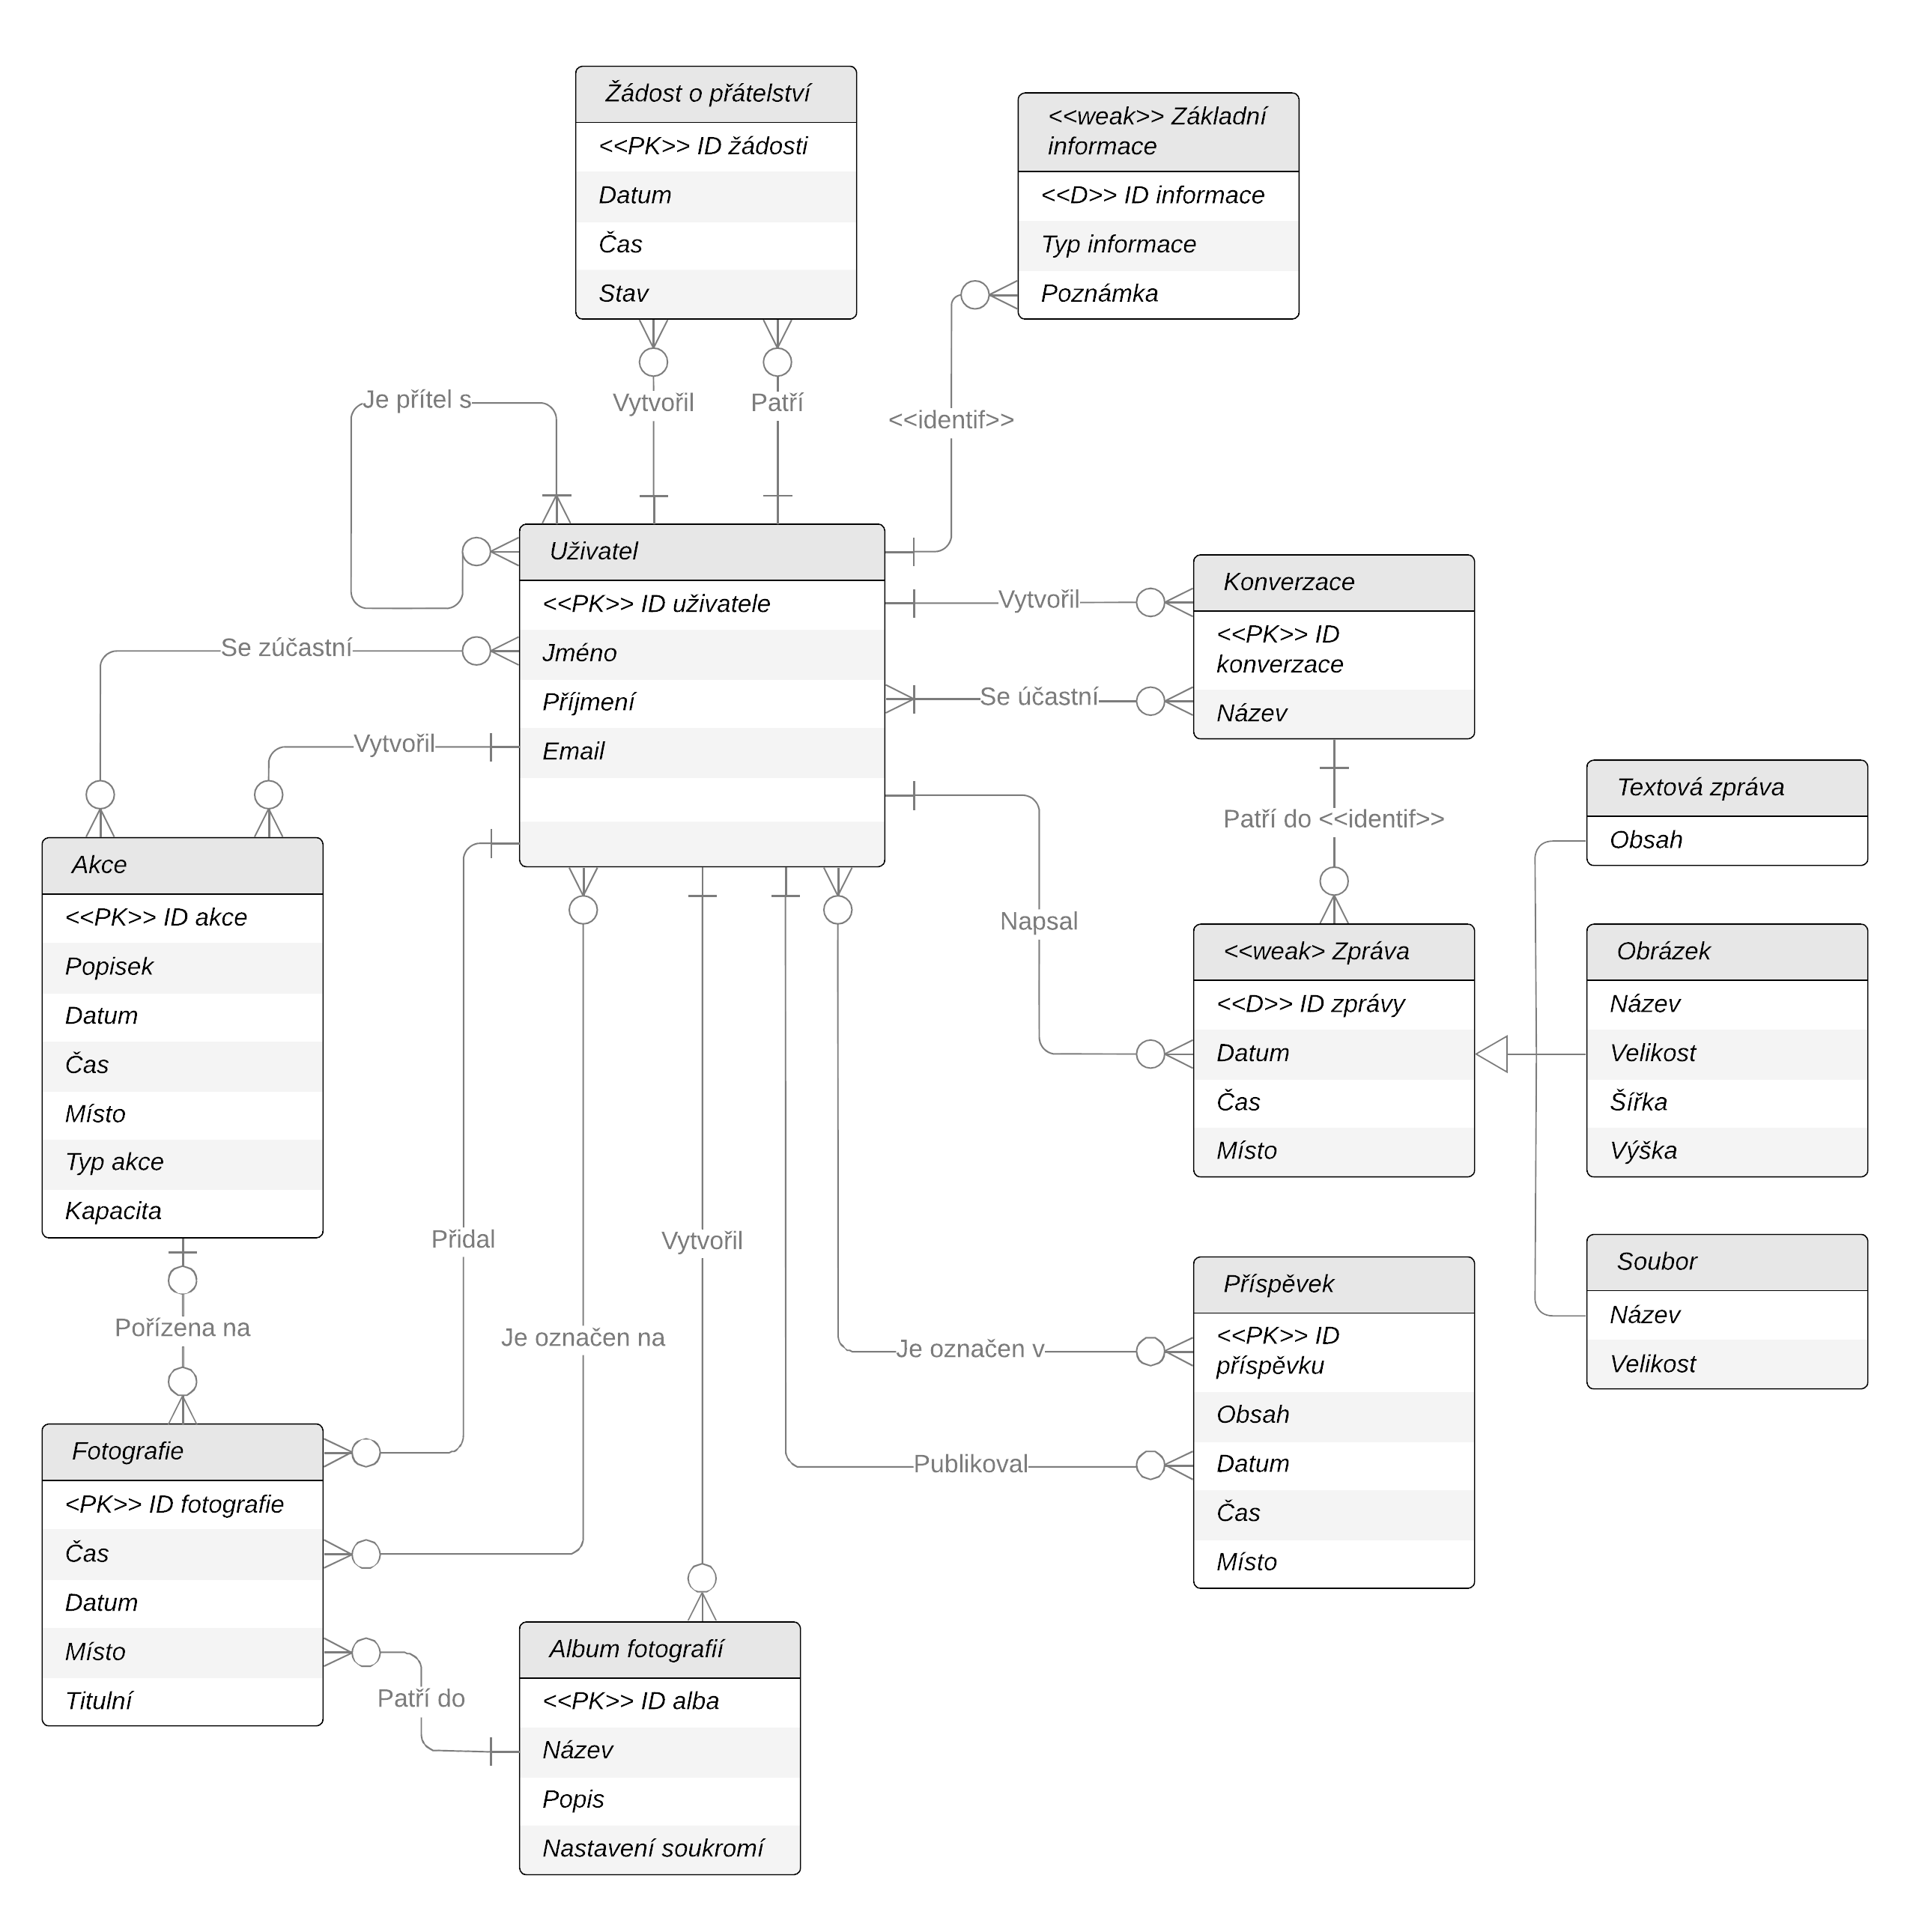
\includegraphics[width=\textwidth]{ERD}
  \caption{ERD Diagram}
\end{figure}

\begin{figure}[H]
  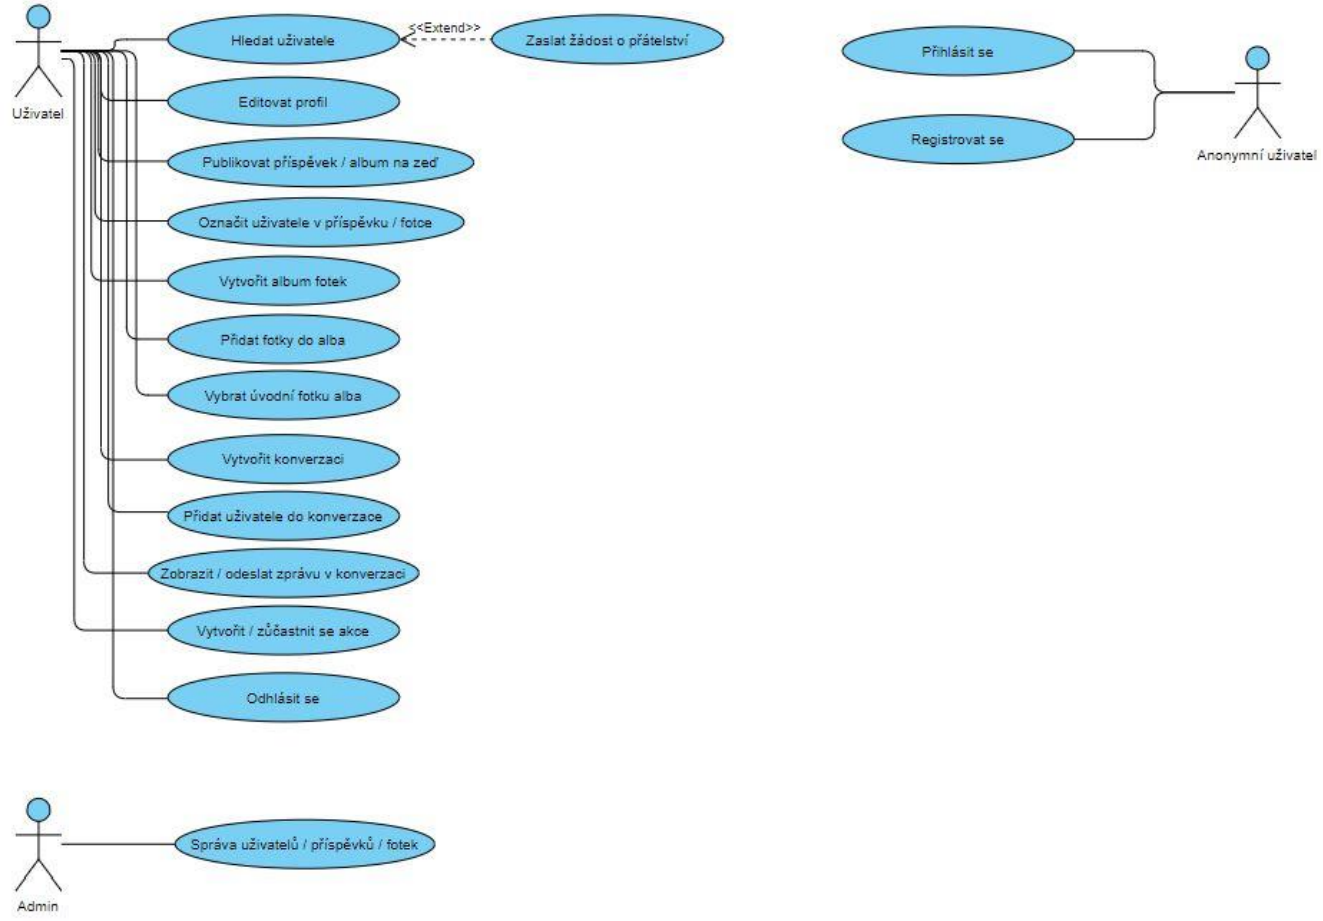
\includegraphics[width=\textwidth]{UCD}
  \caption{Use Case Diagram}
\end{figure}

\section{Vytvoření základních objektů schématu databáze}

\section{SQL dotazy SELECT}

\subsection{Spojení dvou tabulek}
\begin{minipage}{\linewidth}
    \begin{center}
        \begin{lstlisting}[language=sql]
        -- Jake prispevky publikoval uzivatel
        SELECT jmeno, prijmeni, obsah
        FROM uzivatel U,
             prispevek P
        WHERE U.id = P.autor;
        
        -- Dalsi dotaz
        SELECT U.jmeno, U.prijmeni, I.vzdelani
        FROM uzivatel U,
             zakladni_informace I
        WHERE U.id = I.uzivatel
          AND I.vzdelani IS NOT NULL;\end{lstlisting}
    \end{center}
\end{minipage}

\subsection{Spojení tří tabulek}
\begin{minipage}{\linewidth}
    \begin{center}
        \begin{lstlisting}[language=sql]
        -- Dotaz 1
        SELECT CONCAT(CONCAT(U.jmeno, ' '), U.prijmeni) jmeno
        FROM uzivatel U,
             akce A,
             ucastnici_akce UA
        WHERE U.id = UA.uzivatel
          AND UA.akce = A.id
          AND A.popisek LIKE 'Koncert skupiny XYZ';
          
        -- Dotaz 2
        SELECT CONCAT(CONCAT(U.jmeno, ' '), U.prijmeni) jmeno, F.cesta foto
        FROM uzivatel U,
             foto_oznaceni FO,
             fotografie F
        WHERE U.id = FO.uzivatel
          AND FO.fotografie = F.id
        ORDER BY jmeno;\end{lstlisting}
    \end{center}
\end{minipage}

\subsection{Dotazy s GROUP BY}
\begin{minipage}{\linewidth}
    \begin{center}
        \begin{lstlisting}[language=sql]
        -- Prvni dotaz
        SELECT A.nazev, COUNT(*) AS pocet_fotek_v_albumu
        FROM album A,
             fotografie F
        WHERE A.id = F.album
        GROUP BY A.nazev;
        
        -- Druhy dotaz
        SELECT popisek, COUNT(*) pocet_fotek
        FROM akce A,
             fotografie F
        WHERE A.id = F.akce
        GROUP BY popisek;\end{lstlisting}
    \end{center}
    
    \subsection{Dotaz s predikátem EXISTS}
    \begin{center}
        \begin{lstlisting}[language=sql]
        -- Predikat EXISTS
        SELECT DISTINCT jmeno, prijmeni
        FROM uzivatel U,
             zakladni_informace I
        WHERE U.id = I.uzivatel
          AND vzdelani IS NOT NULL
          AND EXISTS(SELECT *
                     FROM zakladni_informace I
                     WHERE U.id = I.uzivatel
                        AND povolani IS NULL);\end{lstlisting}
    \end{center}
\end{minipage}

\subsection{Dotaz s predikátem IN}
\begin{minipage}{\linewidth}
    \begin{center}
        \begin{lstlisting}[language=sql]
        -- Predikat IN
        SELECT U.jmeno, U.prijmeni
        FROM uzivatel U
        WHERE U.id IN (SELECT zakladatel FROM konverzace);\end{lstlisting}  
    \end{center}
\end{minipage}

\section{Pokročilé objektů schématu databáze}
    \subsection{Triggery}
    \subsection{Procedury}
    \subsection{EXPLAIN PLAN a INDEX}
    \subsection{Přístupová práva}
    \subsection{Matezializovaný pohled}

\section{Závěr}

\end{document}
